\documentclass[12pt,letterpaper]{article}

\usepackage[utf8]{inputenc}
\usepackage[spanish]{babel}
\usepackage{times}
\usepackage[left=3cm,top=2.5cm,bottom=2.5cm,right=2.5cm]{geometry}
\usepackage{graphicx}
\title{EV\_ 2\_ 7\_ Diseño de un Modulación de ancho de pulso (PWM).}


\begin{document}
\maketitle




\paragraph{ UNIVERSIDAD POLITÉCNICA DE LA ZONA METROPOLITANA DE GUADALAJARA}

\
\begin{figure}[h!]
\begin{center}


\includegraphics[scale=0.8]{Upzmg.png} 
\label{Upzmg}


\end{center}
\end{figure}


\

\large{Perez de Alba Santiago Eduardo.\\
Fecha: 22 de Octubre del 2019.
\

Curso: Sep-Nov 2019.

\
Carrera: Ingeniería en Mecatronica.\

Docente: Moran Garabito Carlos Enrique}

\newpage

\section{Modulación de Ancho de Pulso(PWM):}
\
Es una técnica en la cual se modifica el ciclo de trabajo de una señal periódica (tipicamente se emplea sobre señales sinusoidales o cuadradas), ya sea para transmitir información a través de un canal de comunicaciones o para controlar la cantidad de energía que se envía a una determinada carga.
La modulación de ancho de pulso(PWM) de una señal es una técnica que logra producir el efecto de una señal analógica sobre una carga, a partir de una variación de la frecuencia y ciclo de trabajo de una señal digital. El ciclo de trabajo describe la cantidad de tiempo que la señal está en un estado lógico alto, como un porcentaje del tiempo total que este toma para completar un ciclo completo. La frecuencia determina que tan rápido se completa un ciclo, por lo tanto es que tan rápido se cambia entre los estados lógicos alto y bajo. Al cambiar la señal de un estado alto a bajo a una tasa lo suficientemente rápida y con cierto ciclo de trabajo, la salida parecerá comportarse como una señal analógica constante cuando esta está siendo aplicada a algún dispositivo.
\

Se usan inversores DC/AC monofásicos y trifásicos. Se basan en la comparación de una señal de referencia modular y una señal portadora de forma triangular o diente de sierra.
\

\begin{figure}[h!]
\begin{center}

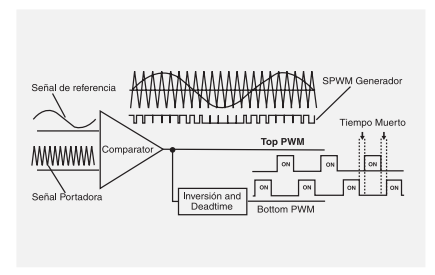
\includegraphics[scale=0.8]{PWM.png} 
\caption{Modulación escalar PWM y SPWM}
\end{center}
\end{figure}
\

La comparación generara un tren de pulsos de ancho especifico que se utilizan en la conmutación del puente inversor. La relación entre la amplitud de la señal portadora y la señal de referencia se le llama "Indice de modulación" y es representada por $m_a$(1), mientras que Ar es la amplitud de la señal de referencia y Ac es la amplitud de la señal portadora. Este indice de modulación permite obtener una tension variable a la salida del inversos.
\

$$m_a = \frac{A_r}{A_c}(1)$$
\
$$m_f = \frac{F_r}{F_c}(2)$$
\

La relación entre la frecuencia de la señal portadora y la frecuencia de referencia es denominada "Indice de frecuencia" y se representa por "$m_r$"(2).
\

El indice de frecuencia determina la distorsión armónica de la señal de salida la cual es una medida de su contenido armónico.
\

\

El ciclo de trabajo de una señal periódica \textit{D} se define a través del cociente entre el ancho relativo de su parte positiva \textit{W} y el periodo de la señal \textit{T}.
\

$$D=\frac{W}{T}$$
\
Donde:

\
\textit{D}: Es el denominado ciclo de trabajo(Tipicamente definido en porcentaje).

\
\textit{W}: Es el tiempo en que la función es positiva(ancho del pulso).

\
\textit{T}: Es el período de la señal.

\

\begin{figure}[h!]
\begin{center}
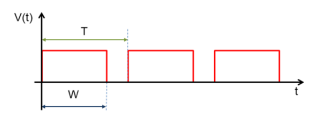
\includegraphics[scale=0.8]{Parametros.png} 
\caption{Parametros \textit{T} y \textit{W} para una señal periódica.}
\end{center}
\end{figure}

\
Sus principales aplicaciones están orientadas fundamentalmente al control de: Fuentes conmutadas, Velocidad de motores, la posición de un servomotor, elementos termoeléctricos, interruptores electrónicos, sensores en ambientes ruidosos, conversores \textit{D/A}




\end{document}